% CSE731 Software Testing - Final Project Report
% Compile with pdflatex (e.g. on Overleaf: upload the docs/report folder).
\documentclass[12pt,a4paper,oneside]{report}

% ---------------------------------------------------------------- packages
\usepackage[T1]{fontenc}
\usepackage[utf8]{inputenc}
\usepackage{lmodern}
\usepackage[a4paper,margin=2.5cm]{geometry}
\usepackage{graphicx}
\usepackage{float}
\usepackage{caption}
\usepackage{booktabs}
\usepackage{tabularx}
\usepackage{longtable}
\usepackage{array}
\usepackage{multirow}
\usepackage[table]{xcolor}
\usepackage{enumitem}
\usepackage{pifont}
\usepackage{titlesec}
\usepackage{tikz}
\usetikzlibrary{positioning,arrows.meta,fit,backgrounds,calc}
\usepackage{pgfplots}
\pgfplotsset{compat=1.17}
\usepackage{listings}
\usepackage[hidelinks]{hyperref}
\hypersetup{colorlinks=true,linkcolor=black,urlcolor=cyan!70!blue,citecolor=black}

% ---------------------------------------------------------------- details
\newcommand{\lecturer}{Prof. Meenakshi D Souza}
\newcommand{\submissiondate}{30/11/2026}
\newcommand{\repourl}{https://github.com/gishee003/Blog-E2E-Testing}

% ---------------------------------------------------------------- styling
\titleformat{\chapter}[block]{\centering\Huge\bfseries}{Chapter \thechapter:}{0.5em}{}
\titlespacing*{\chapter}{0pt}{30pt}{30pt}
\setlength{\parindent}{1.5em}
\setlength{\parskip}{3pt}
\renewcommand{\arraystretch}{1.25}
\captionsetup{font=small}

\newcommand{\pass}{\textcolor{green!50!black}{\ding{51}}}
\newcommand{\fail}{\textcolor{red!75!black}{\ding{55}}}
\newcommand{\na}{--}
\newcommand{\code}[1]{\texttt{#1}}

\definecolor{codebg}{RGB}{246,248,250}
\lstset{
  basicstyle=\ttfamily\footnotesize,
  backgroundcolor=\color{codebg},
  frame=single, rulecolor=\color{black!15},
  breaklines=true, columns=fullflexible,
  keywordstyle=\color{blue!60!black}\bfseries,
  commentstyle=\color{green!40!black}\itshape,
  stringstyle=\color{red!60!black},
  showstringspaces=false, xleftmargin=4pt, xrightmargin=4pt
}
\lstdefinelanguage{JavaScript}{
  keywords={const,let,var,async,await,function,return,if,else,new,throw,try,catch,require,module,exports},
  sensitive=true, comment=[l]{//}, morecomment=[s]{/*}{*/},
  morestring=[b]', morestring=[b]", morestring=[b]`
}

% Bug report block (tabularx must be used as \tabularx...\endtabularx inside
% an environment definition)
\newenvironment{bugreport}[3]{%
  \par\medskip\noindent
  \tabularx{\textwidth}{|>{\bfseries\columncolor{black!6}}p{3.1cm}|X|}
  \hline
  \rowcolor{black!14}\multicolumn{2}{|l|}{\textbf{#1: #2}} \\ \hline
  Severity & #3 \\ \hline
}{%
  \endtabularx\par\medskip
}

\begin{document}

% ================================================================= TITLE PAGE
\begin{titlepage}
  \centering
  {\LARGE\bfseries International Institute of Information\\[4pt] Technology, Bangalore\par}
  \vspace{1.6cm}
  
\includegraphics[width=0.75\textwidth]{figures/iiitb-logo.png}\par
  \vspace{1.6cm}
  {\Large\bfseries CSE 731: Software Testing\par}
  \vspace{0.4cm}
  \rule{0.75\textwidth}{0.6pt}\par
  \vspace{0.3cm}
  {\LARGE Final Project\par}
  \vspace{0.25cm}
  {\large\bfseries End-to-End Testing of a MERN Blog Application\\ with Playwright\par}
  \vspace{0.2cm}
  \rule{0.75\textwidth}{0.6pt}\par
  \vspace{1.2cm}
  \begin{tabular}{ll}
    \textbf{\large Student Name} & \textbf{\large Student ID} \\
    Kirti Nigam & MT2025066 \\
    Athira Lonappan & MT2025027 \\
  \end{tabular}\par
  \vspace{1.2cm}
  {\large\bfseries Lecturer in charge:\par}
  \vspace{0.2cm}
  {\Large {Prof. Meenakshi D Souza}\par}
  \vfill
  {\bfseries Submission Date : 30/11/2026\par}
\end{titlepage}

\pagenumbering{roman}
\tableofcontents
\clearpage
\pagenumbering{arabic}

% ================================================================= CHAPTER 1
\chapter{Introduction}

In this project we tested a web application from end to end using
\textbf{Playwright}. The application is a blog built with the \textbf{MERN}
stack (MongoDB, Express, React and Node.js). On this blog, a user can register,
log in, write posts, edit them and comment on posts. All of these actions are
saved in the database, and most of them need the user to be logged in.

We ran our tests on three browsers: Chromium, Firefox and WebKit. The tests
cover the following areas:

\begin{itemize}[nosep]
  \item \textbf{Main workflows}: registering, logging in, creating and editing
        posts, and adding comments. After each action we also check the
        database to make sure the data was really saved.
  \item \textbf{Negative and edge cases} using \textbf{session-data based
        testing}. The app keeps the login session as a token (JWT) in the
        browser's \code{localStorage}. We changed this token in different ways,
        for example by removing it, editing it, using an expired one or using
        another user's token, and checked how the app reacted.
  \item \textbf{Network failures}, such as a server that cannot be reached, the
        browser going offline, a slow server and server errors.
  \item \textbf{Unauthorized access} and \textbf{form validation errors}.
\end{itemize}

We wrote all the test cases ourselves. We did not use any AI agents or
agent-based testing frameworks to create or run the tests.

\section*{What this report contains}

\begin{tabularx}{\textwidth}{>{\raggedright\arraybackslash}p{6.2cm}X}
\toprule
\textbf{Requirement} & \textbf{Where} \\
\midrule
Application architecture diagram & Chapter~\ref{ch:arch} \\
Testing problems considered & Chapter~\ref{ch:problems} \\
Choice of tools and browser compatibility & Chapter~\ref{ch:tools} \\
List of test cases & Chapter~\ref{ch:cases} \\
Summary of results with pass/fail rates & Chapter~\ref{ch:summary} \\
Bug reports & Chapter~\ref{ch:bugs} \\
Screenshots of the application and tests & Chapter~\ref{ch:screens} \\
Repository (source code, installation, tests) & \href{\repourl}{\nolinkurl{github.com/gishee003/Blog-E2E-Testing}} \\
\bottomrule
\end{tabularx}

% ================================================================= CHAPTER 2
\chapter{Application and Architecture}\label{ch:arch}

\section{The application}

We did not build this application ourselves. We took it from the open-source
repository \href{https://github.com/apirollijr/blog}{\nolinkurl{apirollijr/blog}}
on GitHub (commit \code{5928eab}, ISC licence). We picked it because it has all
three layers of a web application (a React front end, an Express server and a
MongoDB database), it uses token-based login, and every post belongs to a user.
The code is also small, so we were able to read all of it before writing our
tests. Table~\ref{tab:stack} shows the technologies it uses.

\begin{table}[H]
\centering
\begin{tabular}{lll}
\toprule
\textbf{Layer} & \textbf{Technology} & \textbf{Version} \\
\midrule
Front end & React (Create React App), React Router, Axios & 19.1.0, 7.6.3, 1.10.0 \\
Server & Node.js, Express & 22.15.0, 5.1.0 \\
Login & jsonwebtoken (JWT, valid for 7 days), bcryptjs & 9.0.2, 3.0.2 \\
Database access & Mongoose & 8.16.1 \\
Database & MongoDB Community Server & 8.0.9 \\
\bottomrule
\end{tabular}
\caption{Technologies used by the application}
\label{tab:stack}
\end{table}

\subsection*{Changes we made to the front end}

When we downloaded the project, the back end was complete, but four front-end
files were empty: \code{pages/Post.js}, \code{components/PostForm.js},
\code{components/CommentList.js} and \code{components/PostList.js}. Because of
this, the website had no page for a single post, no form to create or edit a
post and no comments section. We could not test any real workflow without these
pages, so we wrote them ourselves. We added:

\begin{itemize}[nosep]
  \item a post page, with Edit and Delete buttons shown only to the author,
  \item a form for creating and editing posts,
  \item a comments section,
  \item a navigation bar with a Logout button,
  \item a check that sends logged-out users to the login page.
\end{itemize}

We also changed the Axios client so that it sends the token with every request
and logs the user out if the server replies with \code{401}.

We did not change the back end or the original Home, Login and Register pages.
This means all the bugs in Chapter~\ref{ch:bugs} come from the original
project and not from our changes. In the repository, every file we added or
changed is marked with the comment \code{[added for E2E project]}.

\section{Architecture}

Figure~\ref{fig:arch} shows the three layers of the application and how our
tests connect to them. Playwright opens real browsers and uses the website the
way a user would. It can also block or change the requests between the browser
and the server, which is how we create network errors. To set up test data,
and for some server checks, it calls the REST API directly. Finally, it
connects to MongoDB to check that the data was really saved.

\begin{figure}[H]
\centering
\resizebox{\textwidth}{!}{%
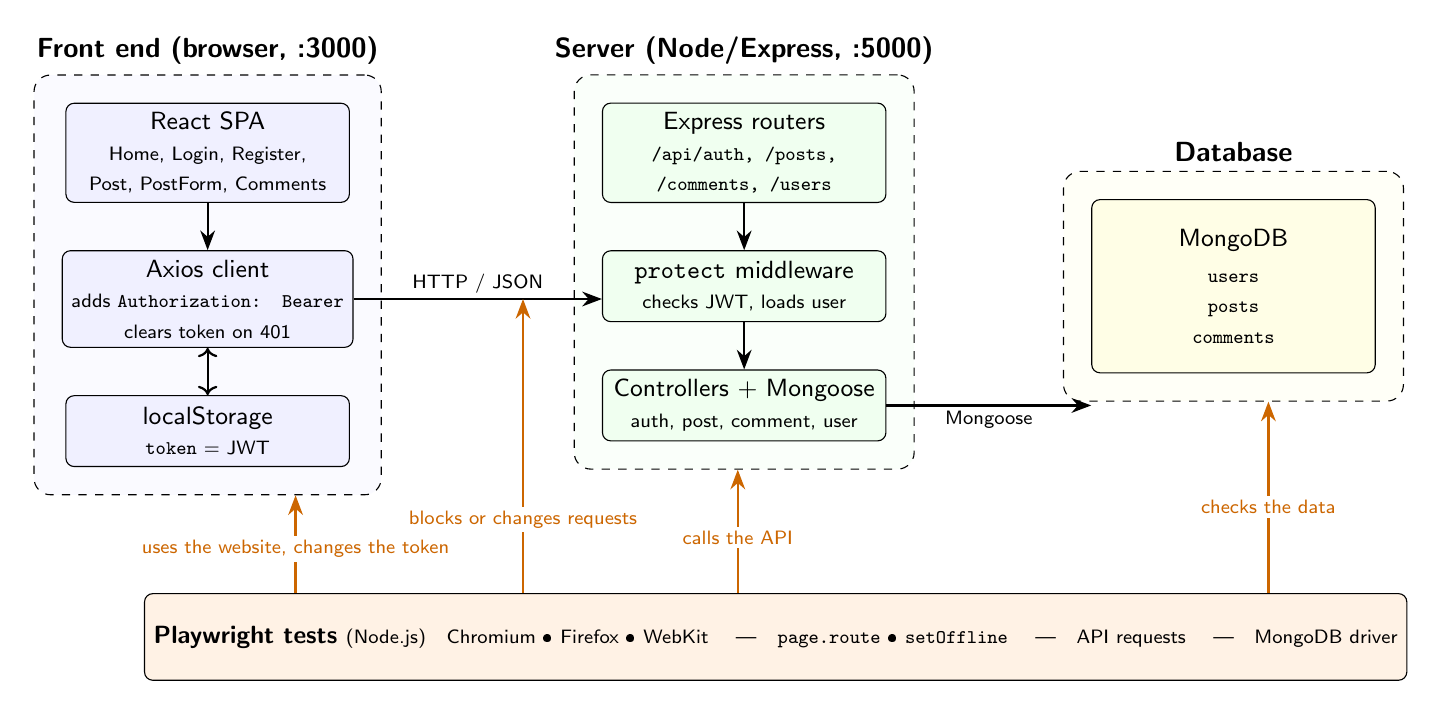
\begin{tikzpicture}[
  font=\sffamily\small,
  box/.style={draw, rounded corners=3pt, align=center, minimum width=3.6cm, minimum height=0.9cm, fill=white},
  tier/.style={draw, rounded corners=6pt, inner sep=10pt, dashed},
  arr/.style={-{Stealth[length=2.5mm]}, thick},
  tarr/.style={-{Stealth[length=2.5mm]}, thick, orange!80!black},
  lbl/.style={font=\sffamily\scriptsize, fill=white, inner sep=1.5pt}
]
% Client tier
\node[box, fill=blue!6] (spa) {React SPA\\\scriptsize Home, Login, Register,\\\scriptsize Post, PostForm, Comments};
\node[box, fill=blue!6, below=0.6cm of spa] (axios) {Axios client\\\scriptsize adds \texttt{Authorization: Bearer}\\\scriptsize clears token on 401};
\node[box, fill=blue!6, below=0.6cm of axios] (ls) {localStorage\\\scriptsize \texttt{token} = JWT};
\draw[arr] (spa) -- (axios);
\draw[arr, <->] (axios) -- (ls);
\begin{scope}[on background layer]
\node[tier, fill=blue!2, fit=(spa)(axios)(ls), label={[font=\sffamily\bfseries]above:{Front end (browser, :3000)}}] (client) {};
\end{scope}

% Server tier
\node[box, fill=green!6, right=3.2cm of spa] (routes) {Express routers\\\scriptsize \texttt{/api/auth, /posts,}\\\scriptsize \texttt{/comments, /users}};
\node[box, fill=green!6, below=0.6cm of routes] (mw) {\texttt{protect} middleware\\\scriptsize checks JWT, loads user};
\node[box, fill=green!6, below=0.6cm of mw] (ctrl) {Controllers + Mongoose\\\scriptsize auth, post, comment, user};
\draw[arr] (routes) -- (mw);
\draw[arr] (mw) -- (ctrl);
\begin{scope}[on background layer]
\node[tier, fill=green!2, fit=(routes)(mw)(ctrl), label={[font=\sffamily\bfseries]above:{Server (Node/Express, :5000)}}] (server) {};
\end{scope}

% Data tier
\node[box, fill=yellow!10, right=2.6cm of mw, minimum height=2.2cm] (db) {MongoDB\\[2pt]\scriptsize\texttt{users}\\\scriptsize\texttt{posts}\\\scriptsize\texttt{comments}};
\begin{scope}[on background layer]
\node[tier, fill=yellow!3, fit=(db), label={[font=\sffamily\bfseries]above:Database}] (data) {};
\end{scope}

\draw[arr] (axios.east) -- node[lbl, above] {HTTP / JSON} (routes.west |- axios.east);
\draw[arr] (ctrl.east) -- node[lbl, below] {Mongoose} (db.west |- ctrl.east);

% Test harness
\node[box, fill=orange!10, minimum width=15.5cm, minimum height=1.1cm, anchor=north]
  (pw) at ($(ls.south -| routes.south) + (0.4,-1.6)$)
  {\textbf{Playwright tests} \scriptsize(Node.js)\quad
   Chromium \textbullet\ Firefox \textbullet\ WebKit \quad|\quad \texttt{page.route} \textbullet\ \texttt{setOffline} \quad|\quad
   API requests \quad|\quad MongoDB driver};
\coordinate (t1) at ($(pw.north west)!0.12!(pw.north east)$);
\coordinate (t2) at ($(pw.north west)!0.30!(pw.north east)$);
\coordinate (t3) at ($(pw.north west)!0.47!(pw.north east)$);
\coordinate (t4) at ($(pw.north west)!0.89!(pw.north east)$);
\draw[tarr] (t1) -- node[lbl, pos=0.45] {uses the website, changes the token} (t1 |- client.south);
\draw[tarr] (t2) -- node[lbl, pos=0.25] {blocks or changes requests} (t2 |- axios.east);
\draw[tarr] (t3) -- node[lbl, pos=0.45] {calls the API} (t3 |- server.south);
\draw[tarr] (t4) -- node[lbl, pos=0.45] {checks the data} (t4 |- data.south);
\end{tikzpicture}}
\caption{Architecture of the application and how the tests connect to it}
\label{fig:arch}
\end{figure}

\section{Database and API}

\begin{table}[H]
\centering
\small
\begin{tabularx}{\textwidth}{lX}
\toprule
\textbf{Collection} & \textbf{Fields} \\
\midrule
\code{users} & \code{username} (unique), \code{email} (unique, lower-case), \code{password} (bcrypt hash), timestamps \\
\code{posts} & \code{title} (required, trimmed), \code{body} (required), \code{author} $\rightarrow$ users, timestamps \\
\code{comments} & \code{text} (required), \code{post} $\rightarrow$ posts, \code{author} $\rightarrow$ users, timestamps \\
\bottomrule
\end{tabularx}
\caption{MongoDB collections}
\end{table}

\begin{table}[H]
\centering
\small
\begin{tabular}{lllc}
\toprule
\textbf{Method} & \textbf{Endpoint} & \textbf{What it does} & \textbf{Login needed} \\
\midrule
POST & \code{/api/auth/register} & create an account, returns a JWT & -- \\
POST & \code{/api/auth/login} & log in, returns a JWT & -- \\
GET & \code{/api/posts}, \code{/api/posts/:id} & list posts / read one post & -- \\
POST & \code{/api/posts} & create a post & yes \\
PUT, DELETE & \code{/api/posts/:id} & edit / delete your own post & yes, author only \\
GET & \code{/api/comments/:postId} & comments on a post & -- \\
POST & \code{/api/comments} & add a comment & yes \\
DELETE & \code{/api/comments/:id} & delete your own comment & yes, author only \\
GET, PUT & \code{/api/users/me} & read / update your profile & yes \\
GET & \code{/api/users}, \code{/api/users/:id} & list users / read one user & -- \\
\bottomrule
\end{tabular}
\caption{REST API of the application}
\end{table}

\subsection*{How login works}

When a user logs in, the server creates a JWT that contains the user's id and
sends it back. The browser saves this token in \code{localStorage} under the
key \code{token}, and sends it with every request in the header
\code{Authorization: Bearer <token>}. On the server, the \code{protect}
middleware checks that the token is valid and not expired, finds the user and
passes it on. For editing and deleting, the server also checks that the
logged-in user is the author of the post or comment.

When the user clicks Logout, the token is only deleted from the browser. The
server is not told about it. So on the browser side, the whole login session
is just one string. This is the main reason we chose session-data based
testing for this application.

% ================================================================= CHAPTER 3
\chapter{Testing Problems Considered}\label{ch:problems}

\section{End-to-end workflows}

These tests follow the same steps a real user would take, using the real
website, server and database:

\begin{enumerate}[nosep]
  \item \textbf{Registration and login}: registering, logging in, entering a
        wrong password, registering with an e-mail that is already used,
        logging out, and the browser's checks on the registration form.
  \item \textbf{Creating and editing data}: publishing a post, editing it,
        deleting it, adding and deleting comments, and making sure that other
        users do not see the Edit and Delete buttons.
  \item \textbf{Complete flow}: one long test where a new user registers, logs
        in, publishes a post, edits it, adds a comment, logs out and then opens
        the post as a visitor.
\end{enumerate}

In every test we check three things: what is shown on the page, which page
the user ends up on, and what is saved in MongoDB. For example, after creating
a post we check that its author in the database is the logged-in user. After
registering, we check that the password is saved as a bcrypt hash and not as
plain text.

\section{Client-side technique: session-data based testing}

In client-side testing, we change the data that the browser sends to the
server, to see whether the server trusts data that it should not trust. For
this project we used \textbf{session-data based testing}. We took the login
token that the browser stores and changed it in different ways. After each
change we checked three things:

\begin{enumerate}[nosep]
  \item the status code the server returned,
  \item what the website did next,
  \item whether anything changed in the database.
\end{enumerate}

Table~\ref{tab:sessionmut} lists each change we made and the test case we
wrote for it.

\begin{table}[H]
\centering
\small
\begin{tabularx}{\textwidth}{>{\raggedright\arraybackslash}p{4.6cm}X>{\raggedright\arraybackslash}p{1.6cm}}
\toprule
\textbf{Change made to the session} & \textbf{What should happen} & \textbf{Test} \\
\midrule
No token at all & protected pages go to the login page & TC-SES-01 \\
Token edited to another user's id & server rejects it (401) & TC-SES-02 \\
Token that has expired & 401, user has to log in again & TC-SES-03 \\
Token signed with a guessed key & 401, the other user's post is not changed & TC-SES-04 \\
Token with no signature (\code{alg: none}) & 401 & TC-SES-05 \\
User B's real token used on user A's post & 403, A's post is not changed & TC-SES-06 \\
Token of a user who was deleted & 401 & TC-SES-07 \\
Old token used again after logout & 401 & TC-SES-08 \\
Page reload or a second tab & user stays logged in & TC-SES-09 \\
Two separate browser windows & the sessions do not mix & TC-SES-10 \\
Token deleted while the user is typing & save is blocked, typed text is kept & TC-SES-11 \\
Random text instead of a token & detected when the page loads and removed & TC-SES-12 \\
\bottomrule
\end{tabularx}
\caption{Changes made to the session and the test cases for them}
\label{tab:sessionmut}
\end{table}

We wrote a few small helper functions for changing tokens
(\code{e2e-tests/utils/session.js}). When the tests run, Playwright starts the
server with a secret key that we know. Because of this, we can also create
properly signed tokens for special cases, such as a token that has already
expired, or a token for a user that we deleted from the database. Below is one
of these helpers and a short part of a test that uses it:

\begin{lstlisting}[language=JavaScript]
// Keeps the header and signature, but puts another user's id in the payload
function tamperPayload(token, newUserId) {
  const [header, , signature] = token.split('.');
  const payload = Buffer.from(JSON.stringify({ id: newUserId })).toString('base64url');
  return `${header}.${payload}.${signature}`;
}
// In the test: save the edited token, submit the form, then check server, page and DB
await plantToken(page, S.tamperPayload(attacker.token, victim.id));
const res = await submitNewPost(page, title);
expect(res.status()).toBe(401);
await expectSessionEnded(page);                       // back on login page, token removed
expect(await findPostsByTitle(title)).toHaveLength(0); // nothing was saved
\end{lstlisting}

\section{Network failures}

We created network problems from the test code, without changing the
application. Playwright can stop or change any request (\code{page.route}),
and it can switch the browser offline (\code{context.setOffline}). Our tests
cover these situations:

\begin{itemize}[nosep]
  \item the server refuses the connection while the user publishes a post,
  \item the browser goes offline while adding a comment and then comes back online,
  \item the list of posts fails to load on the home page,
  \item the server is slow (2 seconds) and the user clicks Publish twice,
  \item the server returns a 500 error during login,
  \item the connection drops during login,
  \item the server returns a 503 error while saving an edit.
\end{itemize}

In each case we check that the user sees a message, that what they typed is
not lost, and that no half-saved or duplicate data ends up in the database.

\section{Unauthorized access and form validation}

The session tests above already cover most unauthorized access cases. We also
added an API test that calls every protected endpoint without a token and
expects a 401 reply.

For form validation, we tested empty fields, a wrong e-mail format, input with
only spaces, the 150-character limit on titles, and wrong or non-existent post
ids in the URL. Checks done in the browser can be skipped easily by sending a
request directly to the server. So we also sent the same wrong input straight
to the API, to see whether the server rejects it on its own.

\section{How we set up the tests}

\begin{itemize}[nosep]
  \item \textbf{Separate database}: the tests use their own database,
        \code{blog\_e2e}, which is emptied before every run. Our normal
        development data is never touched.
  \item \textbf{Independent tests}: each test creates its own users and posts
        with unique names, so the tests can run in any order.
  \item \textbf{Quick setup}: data that a test needs beforehand (users, posts,
        comments) is created through the API. Only the part being tested is
        done through the website.
  \item \textbf{Stable locators}: we find elements by their role, label,
        placeholder or \code{data-testid}, not by CSS classes or position.
  \item \textbf{Production build}: we test the built version of the React app.
        The development server reloads the page when the network changes,
        which made our offline tests unreliable.
  \item \textbf{Tests expect the correct behaviour}: if the app does something
        wrong, the test fails. We did not change any test to match wrong
        behaviour. Every failure is listed as a bug in Chapter~\ref{ch:bugs}.
\end{itemize}

% ================================================================= CHAPTER 4
\chapter{Tools and Test Environment}\label{ch:tools}

\section{Choice of tool}

For this project we could use Playwright, Selenium or Cypress, along with
Postman if needed. The table below compares them on the things we needed.

\begin{table}[H]
\centering
\small
\begin{tabularx}{\textwidth}{>{\raggedright\arraybackslash}p{3.4cm}>{\raggedright\arraybackslash}X>{\raggedright\arraybackslash}X>{\raggedright\arraybackslash}X}
\toprule
\textbf{What we needed} & \textbf{Playwright} & \textbf{Cypress} & \textbf{Selenium} \\
\midrule
Several browsers & Chromium, Firefox and WebKit with the same code & Chromium and Firefox; no WebKit & all browsers, through drivers \\
Network failures & built in (\code{route.abort}, \code{route.fulfill}, \code{setOffline}) & \code{cy.intercept} & needs a proxy or extra setup \\
Session data & direct access to \code{localStorage}; several separate sessions in one test & one tab per test & possible, but more code \\
API testing & built-in API requests & \code{cy.request} & needs a separate tool \\
Reports & HTML report with traces, screenshots and video & dashboard or plugins & third-party reporters \\
Waiting & waits automatically before each action & waits automatically & waits must be written by hand \\
\bottomrule
\end{tabularx}
\caption{Comparison of the allowed testing tools}
\end{table}

We chose \textbf{Playwright} because it could do everything we needed in one
tool. The same tests run on Chromium, Firefox and WebKit, which gave us the
browser compatibility results below. It can block or fake any request and put
the browser offline. It can also open two separate browser sessions inside one
test, which we needed to check that sessions do not mix.

Playwright can also send API requests by itself, so we did not need
\textbf{Postman}. Our API tests are saved in the same project and run together
with the browser tests. Along with Playwright, we used the MongoDB Node.js
driver to check the database and the \code{jsonwebtoken} library to create
test tokens.

\section{Test environment}

\begin{table}[H]
\centering
\small
\begin{tabular}{ll}
\toprule
\textbf{Item} & \textbf{Value} \\
\midrule
Operating system & Windows 11 Home \\
Node.js / npm & 22.15.0 / 10.9.2 \\
MongoDB & 8.0.9 (running locally), test database \code{blog\_e2e} \\
Playwright (\code{@playwright/test}) & 1.65.1 \\
How tests run & headless, one at a time (shared database), no retries \\
Saved when a test fails & screenshot, video and Playwright trace \\
Application & API on port 5000, React build on port 3000 \\
\bottomrule
\end{tabular}
\caption{Test environment}
\end{table}

\section{Browser compatibility}

We ran the 39 browser test cases on all three browsers. The 9 API test cases do
not need a browser, so they ran only once.

\begin{table}[H]
\centering
\small
\begin{tabular}{llcccr}
\toprule
\textbf{Project} & \textbf{Browser (version)} & \textbf{Tests} & \textbf{Passed} & \textbf{Failed} & \textbf{Time} \\
\midrule
chromium & Chromium 159.0.8154.6 (Desktop Chrome) & 39 & 33 & 6 & 66.9\,s \\
firefox  & Firefox 159.0 (Desktop Firefox) & 39 & 33 & 6 & 171.3\,s \\
webkit   & WebKit 27.2 (Desktop Safari) & 39 & 33 & 6 & 171.8\,s \\
api      & -- (no browser) & 9 & 1 & 8 & 2.8\,s \\
\bottomrule
\end{tabular}
\caption{Results on each browser (time is the total time of all tests)}
\label{tab:browsers}
\end{table}

The results were the same on all three browsers. The same 33 tests passed and
the same 6 failed on each one, so none of the bugs depend on the browser. All
the failures come from the server or from the app's own logic. Browser form
checks (\code{required}, \code{type="email"}, \code{maxlength}),
\code{localStorage}, \code{alert} and \code{confirm} pop-ups and offline mode
all worked the same way everywhere. Firefox and WebKit took about 2.6 times
longer than Chromium, mostly because these browsers take longer to start for
each test.

We did find one difference between the browsers, but it was in Playwright and
not in the app. In Chromium, Playwright got stuck when it tried to close an
\code{alert()} pop-up while the browser was offline. So we changed TC-NET-06 to
cut off only the login request (\code{route.abort('internetdisconnected')})
instead of putting the whole browser offline. TC-NET-02 still tests full
offline mode.

% ================================================================= CHAPTER 5
\chapter{Test Cases}\label{ch:cases}

Table~\ref{tab:cases} lists all 48 test cases. The last three columns show the
result in Chromium (C), Firefox (F) and WebKit (W). The API tests run without a
browser, so they have only one result. For tests that failed, the expected
result column also shows the bug that the test found.

{\small
\setlength{\LTpre}{6pt}
\begin{longtable}{>{\raggedright\arraybackslash}p{1.7cm}>{\raggedright\arraybackslash}p{5.0cm}>{\raggedright\arraybackslash}p{4.9cm}ccc}
\caption{List of test cases}\label{tab:cases}\\
\toprule
\textbf{ID} & \textbf{Test case} & \textbf{Expected result} & \textbf{C} & \textbf{F} & \textbf{W} \\
\midrule
\endfirsthead
\toprule
\textbf{ID} & \textbf{Test case} & \textbf{Expected result} & \textbf{C} & \textbf{F} & \textbf{W} \\
\midrule
\endhead
\midrule \multicolumn{6}{r}{\footnotesize continued on next page} \\
\endfoot
\bottomrule
\endlastfoot
\multicolumn{6}{l}{\textbf{Registration and login} (\code{01-auth.spec.js})} \\
TC-AUTH-01 & Register a new user & goes to login page; user saved with a hashed password & \pass & \pass & \pass \\
TC-AUTH-02 & Log in with the correct details & goes to home page, token saved, Logout shown & \pass & \pass & \pass \\
TC-AUTH-03 & Log in with a wrong password & ``Invalid credentials'', no token & \pass & \pass & \pass \\
TC-AUTH-04 & Register with an e-mail that is already used & ``User already exists'', still only one user in DB & \pass & \pass & \pass \\
TC-AUTH-05 & Log out & token removed, Login link shown & \pass & \pass & \pass \\
TC-AUTH-06 & Submit an empty or wrong registration form & browser stops it, nothing sent to server & \pass & \pass & \pass \\
\midrule
\multicolumn{6}{l}{\textbf{Posts and comments} (\code{02-posts.spec.js})} \\
TC-POST-01 & Create a post & post page shown, saved in DB with user as author, listed on home page & \pass & \pass & \pass \\
TC-POST-02 & Edit your own post & new title and body shown and saved & \pass & \pass & \pass \\
TC-POST-03 & Open someone else's post & no Edit or Delete buttons & \pass & \pass & \pass \\
TC-POST-04 & Delete your own post & goes to home page, post removed from DB (BUG-01) & \fail & \fail & \fail \\
TC-POST-05 & Add a comment & comment shown with author name and saved & \pass & \pass & \pass \\
TC-POST-06 & Delete your own comment & comment removed from page and DB (BUG-02) & \fail & \fail & \fail \\
TC-POST-07 & Complete flow: register, log in, publish, edit, comment, log out & every step works; final data saved in DB & \pass & \pass & \pass \\
\midrule
\multicolumn{6}{l}{\textbf{Session-data based} (\code{03-session.spec.js})} \\
TC-SES-01 & Open protected pages with no token & goes to login page & \pass & \pass & \pass \\
TC-SES-02 & Token edited to another user's id & 401, logged out, nothing saved & \pass & \pass & \pass \\
TC-SES-03 & Expired token & 401, logged out, nothing saved & \pass & \pass & \pass \\
TC-SES-04 & Forged token used to edit another user's post & 401, post not changed & \pass & \pass & \pass \\
TC-SES-05 & Token with no signature (\code{alg: none}) & 401, nothing saved & \pass & \pass & \pass \\
TC-SES-06 & User B tries to edit user A's post & 403 shown, B stays logged in, post not changed & \pass & \pass & \pass \\
TC-SES-07 & Token of a deleted user & 401, logged out (BUG-03) & \fail & \fail & \fail \\
TC-SES-08 & Old token used again after logout & 401, nothing saved (BUG-04) & \fail & \fail & \fail \\
TC-SES-09 & Reload page and open a second tab & still logged in in both & \pass & \pass & \pass \\
TC-SES-10 & Two separate browser windows & sessions do not mix & \pass & \pass & \pass \\
TC-SES-11 & Token removed while typing, then save & 401 message, typed text kept, nothing saved & \pass & \pass & \pass \\
TC-SES-12 & Random text as token when page loads & 401 detected, token removed, goes to login & \pass & \pass & \pass \\
\midrule
\multicolumn{6}{l}{\textbf{Network failures} (\code{04-network.spec.js})} \\
TC-NET-01 & Publish while the server refuses the connection & error shown, draft kept, nothing saved & \pass & \pass & \pass \\
TC-NET-02 & Comment while offline, then go back online & error shown; works after going online & \pass & \pass & \pass \\
TC-NET-03 & Home page when posts fail to load & an error message is shown (BUG-12) & \fail & \fail & \fail \\
TC-NET-04 & Slow server (2\,s) and Publish clicked twice & button disabled while saving, only one post saved & \pass & \pass & \pass \\
TC-NET-05 & Login gets a 500 error & server message shown, not logged in & \pass & \pass & \pass \\
TC-NET-06 & Connection drops during login & ``Login failed'', not logged in & \pass & \pass & \pass \\
TC-NET-07 & 503 error while saving an edit & message shown, post not changed & \pass & \pass & \pass \\
\midrule
\multicolumn{6}{l}{\textbf{Form validation and edge cases} (\code{05-validation.spec.js})} \\
TC-VAL-01 & Empty title or body & browser stops it, nothing sent & \pass & \pass & \pass \\
TC-VAL-02 & Title with only spaces & error shown, nothing saved & \pass & \pass & \pass \\
TC-VAL-03 & Type 160 characters in the title & field accepts only 150 & \pass & \pass & \pass \\
TC-VAL-04 & Clear the title while editing & browser stops it, post not changed & \pass & \pass & \pass \\
TC-VAL-05 & Comment with only spaces & not saved (BUG-11) & \fail & \fail & \fail \\
TC-VAL-06 & Invalid post id in the URL & error shown & \pass & \pass & \pass \\
TC-VAL-07 & Post id that does not exist & ``Post not found'' & \pass & \pass & \pass \\
\midrule
\multicolumn{6}{l}{\textbf{Server checks, no browser} (\code{api/server-checks.spec.js})} \\
TC-API-01 & Protected endpoints called without a token & 401 for all six & \multicolumn{3}{c}{\pass} \\
TC-API-02 & Register with missing fields & 400 (BUG-07) & \multicolumn{3}{c}{\fail} \\
TC-API-03 & Create a post with a blank title & 400 (BUG-07) & \multicolumn{3}{c}{\fail} \\
TC-API-04 & Update a post with an empty title & 400 (BUG-09) & \multicolumn{3}{c}{\fail} \\
TC-API-05 & Invalid post id & 400 or 404 (BUG-08) & \multicolumn{3}{c}{\fail} \\
TC-API-06 & Empty comment & 400 (BUG-07) & \multicolumn{3}{c}{\fail} \\
TC-API-07 & Comment on a post that does not exist & 404 (BUG-10) & \multicolumn{3}{c}{\fail} \\
TC-API-08 & Contents of an error response & no stack trace (BUG-05) & \multicolumn{3}{c}{\fail} \\
TC-API-09 & \code{GET /api/users} without logging in & 401 (BUG-06) & \multicolumn{3}{c}{\fail} \\
\end{longtable}
}

% ================================================================= CHAPTER 6
\chapter{Test Results Summary}\label{ch:summary}

We ran the full test suite on 26 November 2026 using the command
\code{npx playwright test}. It took 8.8 minutes and ran \textbf{126 tests} in
total (39 browser test cases on 3 browsers, plus 9 API test cases).

\begin{table}[H]
\centering
\begin{tabular}{lrrrr}
\toprule
 & \textbf{Run} & \textbf{Passed} & \textbf{Failed} & \textbf{Pass rate} \\
\midrule
All test runs & 126 & 100 & 26 & 79.4\,\% \\
Test cases (counted once) & 48 & 34 & 14 & 70.8\,\% \\
\bottomrule
\end{tabular}
\caption{Overall result}
\end{table}

\begin{table}[H]
\centering
\begin{tabular}{lcrrrr}
\toprule
\textbf{Group} & \textbf{Cases} & \textbf{Runs} & \textbf{Passed} & \textbf{Failed} & \textbf{Pass rate} \\
\midrule
Registration and login & 6 & 18 & 18 & 0 & 100.0\,\% \\
Posts and comments & 7 & 21 & 15 & 6 & 71.4\,\% \\
Session-data based & 12 & 36 & 30 & 6 & 83.3\,\% \\
Network failures & 7 & 21 & 18 & 3 & 85.7\,\% \\
Form validation and edge cases & 7 & 21 & 18 & 3 & 85.7\,\% \\
Server checks (API) & 9 & 9 & 1 & 8 & 11.1\,\% \\
\midrule
\textbf{Total} & \textbf{48} & \textbf{126} & \textbf{100} & \textbf{26} & \textbf{79.4\,\%} \\
\bottomrule
\end{tabular}
\caption{Results for each group of tests}
\end{table}

\begin{figure}[H]
\centering
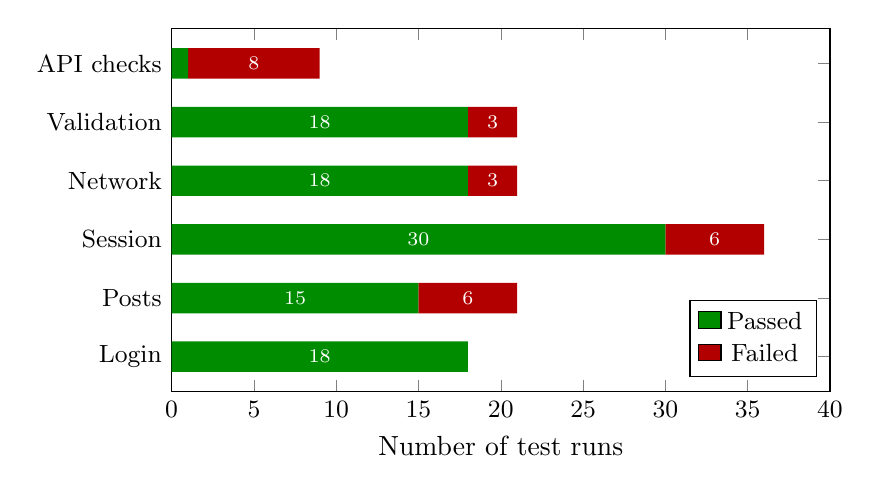
\begin{tikzpicture}
\begin{axis}[
  xbar stacked, width=0.82\textwidth, height=6.2cm,
  bar width=11pt, xmin=0, xmax=40,
  xlabel={Number of test runs},
  symbolic y coords={API checks,Validation,Network,Session,Posts,Login},
  ytick=data, y dir=reverse,
  legend style={at={(0.98,0.04)}, anchor=south east, font=\small},
  nodes near coords, nodes near coords style={font=\scriptsize, color=white},
  point meta=explicit symbolic,
  enlarge y limits=0.12,
  tick label style={font=\small}
]
\addplot[fill=green!55!black, draw=none] coordinates
  {(18,Login)[18] (15,Posts)[15] (30,Session)[30] (18,Network)[18] (18,Validation)[18] (1,API checks)[]};
\addplot[fill=red!70!black, draw=none] coordinates
  {(0,Login)[] (6,Posts)[6] (6,Session)[6] (3,Network)[3] (3,Validation)[3] (8,API checks)[8]};
\legend{Passed, Failed}
\end{axis}
\end{tikzpicture}
\caption{Passed and failed test runs in each group}
\end{figure}

\section*{What the results show}

Every failure is caused by a real bug in the application. In the final run, no
test failed because of timing or because of the test setup, and each failure
happened on every browser. The 14 failed test cases point to 12 different bugs
(Chapter~\ref{ch:bugs}). Three of them come from the same bug, BUG-07.

Registration and login work correctly. The main session checks also work: the
server rejects edited, forged, unsigned and expired tokens, and one user cannot
edit another user's post. The weakest part of the app is how the server handles
wrong input. 8 out of 9 API tests failed, and in most of them the server
returned a 500 error instead of a 400 or 404.

\section*{Problems we fixed while writing the tests}

We found two problems while building the tests and fixed them before the final
run, so they are not counted in the results above. The first was in the edit
form that we wrote: the user could start typing before the post had finished
loading, and then the loaded text replaced what they had typed. We fixed this
by disabling the form until the post is loaded. The second was the Chromium
pop-up problem described in Chapter~\ref{ch:tools}, which we fixed in the test.

\begin{figure}[H]
\centering
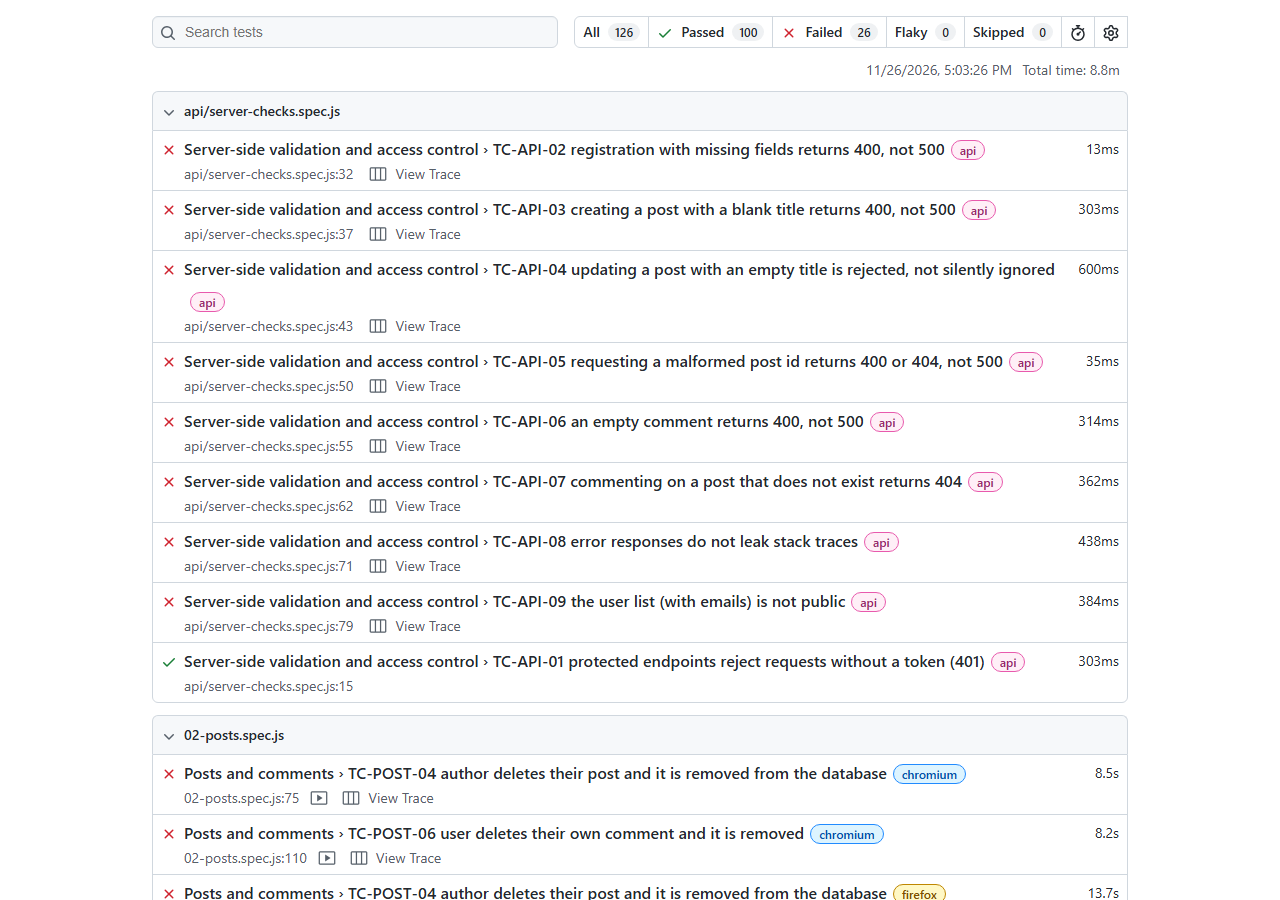
\includegraphics[width=0.92\textwidth]{figures/report-overview.png}
\caption{Playwright HTML report: 126 tests, 100 passed, 26 failed}
\end{figure}

\begin{figure}[H]
\centering
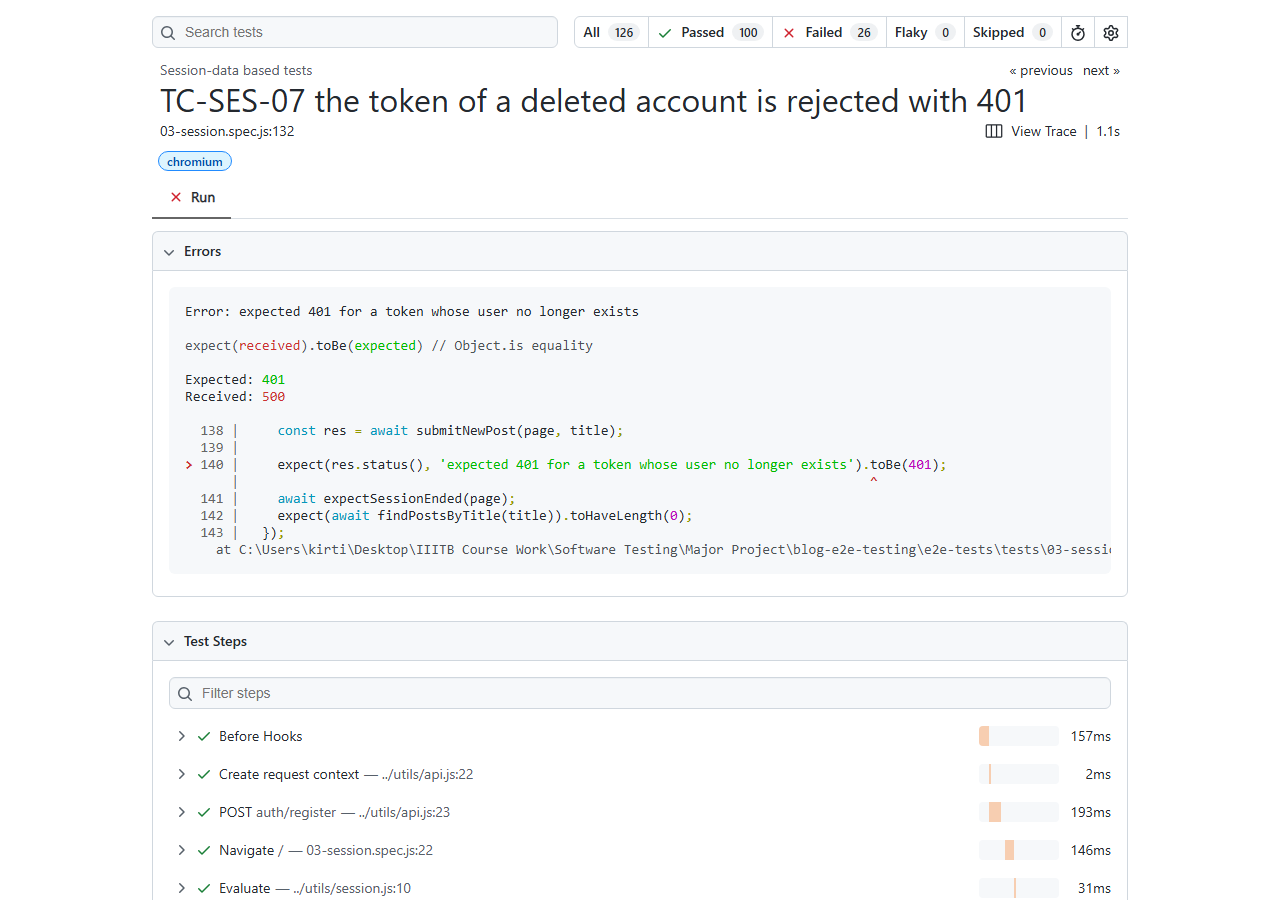
\includegraphics[width=0.92\textwidth]{figures/report-failure-detail.png}
\caption{Details of the failed test TC-SES-07: expected 401, received 500}
\end{figure}

% ================================================================= CHAPTER 7
\chapter{Bug Reports}\label{ch:bugs}

We gave each bug a severity level:

\begin{itemize}[nosep]
  \item \textbf{High}: a main feature does not work at all.
  \item \textbf{Medium}: a security, privacy or data problem.
  \item \textbf{Low}: a wrong status code or a small usability problem.
\end{itemize}

Every bug happened on Chromium 159, Firefox 159 and WebKit 27.2 (API bugs were
tested directly over HTTP), using the original code at commit \code{5928eab}.

\begin{table}[H]
\centering
\small
\begin{tabularx}{\textwidth}{llXl}
\toprule
\textbf{ID} & \textbf{Severity} & \textbf{Summary} & \textbf{Found by} \\
\midrule
BUG-01 & High & Deleting a post always fails with a 500 error & TC-POST-04 \\
BUG-02 & High & Deleting a comment always fails with a 500 error & TC-POST-06 \\
BUG-03 & Medium & A deleted user's token gives a 500 error instead of 401 & TC-SES-07 \\
BUG-04 & Medium & A token still works after logout & TC-SES-08 \\
BUG-05 & Medium & Error replies show stack traces and server file paths & TC-API-08 \\
BUG-06 & Medium & Anyone can see the list of all users with their e-mails & TC-API-09 \\
BUG-07 & Medium & Missing or blank fields give a 500 error with raw database messages & TC-API-02, 03, 06 \\
BUG-08 & Low & An invalid id gives a 500 error instead of 400 or 404 & TC-API-05 \\
BUG-09 & Low & An empty title in an update is ignored without any error & TC-API-04 \\
BUG-10 & Medium & Comments can be added to posts that do not exist & TC-API-07 \\
BUG-11 & Low & Comments with only spaces are saved & TC-VAL-05 \\
BUG-12 & Low & Home page shows nothing, and no error, when posts fail to load & TC-NET-03 \\
\bottomrule
\end{tabularx}
\caption{List of bugs found}
\end{table}

\begin{bugreport}{BUG-01}{Deleting a post always fails}{High}
Component & \code{controllers/postController.js}, \code{deletePost} \\ \hline
Steps & 1. Log in and open one of your own posts. 2. Click \emph{Delete} and confirm. \\ \hline
Expected & The post is deleted from the database and the user goes to the home page. \\ \hline
Actual & The server returns 500 \code{\{"message":"post.remove is not a function"\}}. The error is shown on the page and the post is not deleted (Figure~\ref{fig:bugdelete}). \\ \hline
Cause & The \code{remove()} method was removed in Mongoose 7, and the app uses Mongoose 8. \\ \hline
Suggested fix & Use \code{await post.deleteOne()} instead. \\ \hline
\end{bugreport}

\begin{bugreport}{BUG-02}{Deleting a comment always fails}{High}
Component & \code{controllers/commentController.js}, \code{deleteComment} \\ \hline
Steps & 1. Log in and add a comment. 2. Click \emph{Delete} next to it. \\ \hline
Expected & The comment is removed from the page and the database. \\ \hline
Actual & The server returns 500 \code{comment.remove is not a function} and the comment stays. \\ \hline
Cause & Same as BUG-01. \\ \hline
Suggested fix & Use \code{await comment.deleteOne()} instead. \\ \hline
\end{bugreport}

\begin{bugreport}{BUG-03}{A deleted user's token causes a server error}{Medium}
Component & \code{middleware/auth.js}, \code{protect} \\ \hline
Steps & 1. Log in. 2. Delete this user from the database. 3. In the same browser, publish a post or open \code{/api/users/me}. \\ \hline
Expected & The server returns 401, and the website logs the user out and shows the login page. \\ \hline
Actual & The server returns 500 \code{Cannot read properties of null (reading '\_id')}. The website keeps the old session and shows a technical error message. \\ \hline
Cause & \code{protect} looks up the user, gets \code{null}, and continues without checking it. \\ \hline
Suggested fix & If the user is not found, return 401 with a message such as ``User no longer exists''. \\ \hline
\end{bugreport}

\begin{bugreport}{BUG-04}{A token still works after logout}{Medium}
Component & Login design (logout only deletes the token in the browser) \\ \hline
Steps & 1. Log in and copy the token from \code{localStorage}. 2. Log out. 3. Put the copied token back and publish a post. \\ \hline
Expected & The token no longer works after logout (401). \\ \hline
Actual & The server returns 201 and the post is created. If someone gets hold of a token, for example on a shared computer, they can keep using it for 7 days until it expires. \\ \hline
Suggested fix & Let the server cancel a token on logout (for example, by keeping a list of logged-out tokens), and make tokens expire sooner. \\ \hline
\end{bugreport}

\begin{bugreport}{BUG-05}{Error replies show stack traces}{Medium}
Component & \code{middleware/errorHandler.js} \\ \hline
Steps & Cause any server error, for example \code{GET /api/users/me} with a deleted user's token. \\ \hline
Expected & A simple error message without internal details. \\ \hline
Actual & The reply contains a \code{stack} field with the full stack trace, including the file paths on the server. \\ \hline
Cause & The stack trace is sent unless \code{NODE\_ENV} is set to \code{production}, and the app never sets it. \\ \hline
Suggested fix & Do not send \code{err.stack} in the reply. Write it to the server log instead. \\ \hline
\end{bugreport}

\begin{bugreport}{BUG-06}{Anyone can see all users and their e-mails}{Medium}
Component & \code{routes/users.js}, \code{GET /api/users} \\ \hline
Steps & Without logging in, open \code{GET /api/users}. \\ \hline
Expected & 401, or a list that does not include personal details. \\ \hline
Actual & The server returns 200 with every user's username, e-mail address and dates. \\ \hline
Suggested fix & Allow this route only for admins, and do not return e-mail addresses publicly. \code{GET /api/users/:id} has the same problem. \\ \hline
\end{bugreport}

\begin{bugreport}{BUG-07}{Wrong input gives a 500 error with raw database messages}{Medium}
Component & \code{authController.register}, \code{postController.createPost}, \code{commentController.createComment} \\ \hline
Steps & Send \code{POST /api/auth/register} with only an e-mail, \code{POST /api/posts} with the title \code{"   "}, or \code{POST /api/comments} with empty text. \\ \hline
Expected & 400 with a clear message for the user. \\ \hline
Actual & 500 with Mongoose's internal message, for example \code{User validation failed: username: Path `username` is required.} The same message is also shown to users on the website. \\ \hline
Suggested fix & Check the input before saving it, and return 400 for validation errors. The project has an empty \code{utils/validator.js} file, so this was probably planned. \\ \hline
\end{bugreport}

\begin{bugreport}{BUG-08}{An invalid id gives a 500 error}{Low}
Component & \code{getPostById} and the other routes that take an \code{:id} \\ \hline
Steps & Open \code{GET /api/posts/not-an-id}. \\ \hline
Expected & 400 or 404. \\ \hline
Actual & 500 \code{Cast to ObjectId failed for value "not-an-id"}. \\ \hline
Suggested fix & Check the id with \code{mongoose.isValidObjectId(id)} first and return 404 if it is not valid. \\ \hline
\end{bugreport}

\begin{bugreport}{BUG-09}{An empty title in an update is ignored}{Low}
Component & \code{postController.updatePost} \\ \hline
Steps & As the author, send \code{PUT /api/posts/:id} with \code{\{"title": ""\}}. \\ \hline
Expected & 400 with a message that the title cannot be empty. \\ \hline
Actual & 200, and the old title is kept. The website thinks the update worked. \\ \hline
Cause & The code \code{post.title = req.body.title || post.title} treats an empty string as if no title was sent. \\ \hline
Suggested fix & Check whether a title was sent, and if it was, check that it is not empty. \\ \hline
\end{bugreport}

\begin{bugreport}{BUG-10}{Comments can be added to posts that do not exist}{Medium}
Component & \code{commentController.createComment} \\ \hline
Steps & While logged in, send \code{POST /api/comments} with a valid-looking \code{postId} that does not belong to any post. \\ \hline
Expected & 404 ``Post not found''. \\ \hline
Actual & 201, and the comment is saved for a post that does not exist. Also, when a post is deleted, its comments are not deleted. \\ \hline
Suggested fix & Check that the post exists before saving the comment, and delete a post's comments when the post is deleted. \\ \hline
\end{bugreport}

\begin{bugreport}{BUG-11}{Comments with only spaces are saved}{Low}
Component & \code{models/Comment.js} \\ \hline
Steps & On a post page, type three spaces in the comment box and click \emph{Add comment}. \\ \hline
Expected & The comment is not accepted. \\ \hline
Actual & An empty-looking comment is saved and shown. \\ \hline
Suggested fix & Add \code{trim: true} to the \code{text} field in the schema, as the post title already has. \\ \hline
\end{bugreport}

\begin{bugreport}{BUG-12}{Home page shows nothing when posts fail to load}{Low}
Component & \code{blog-client/src/pages/Home.js} \\ \hline
Steps & Open the home page while the server is down or the network fails. \\ \hline
Expected & A message such as ``Could not load posts, please try again''. \\ \hline
Actual & Only the heading is shown (Figure~\ref{fig:bughome}). The error is only printed in the browser console, so the user cannot tell whether the server is down or the blog just has no posts. \\ \hline
Suggested fix & Store the error in the Home page and show a message with a Retry button. \\ \hline
\end{bugreport}

% ================================================================= CHAPTER 8
\chapter{Application Test Results}\label{ch:screens}

These screenshots were taken with Playwright in Chromium, using the test
database. The script that takes them is
\code{e2e-tests/scripts/capture-report-figures.js}.

\begin{figure}[H]
\centering
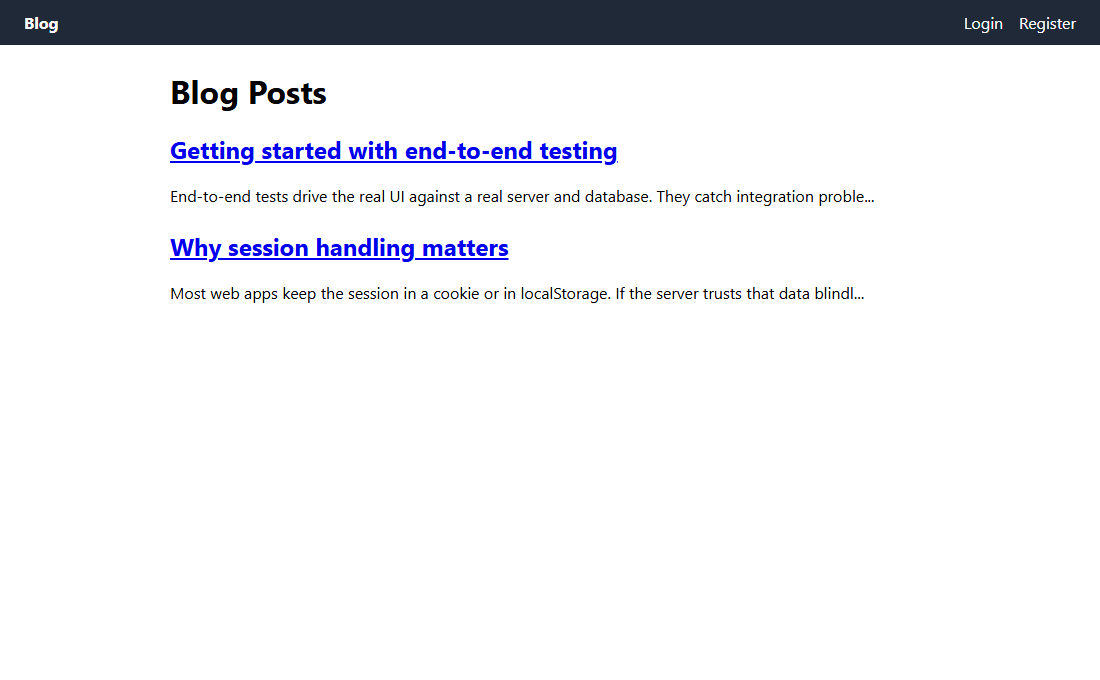
\includegraphics[width=0.85\textwidth]{figures/app-home.png}
\caption{Home page with the list of posts}
\end{figure}

\begin{figure}[H]
\centering
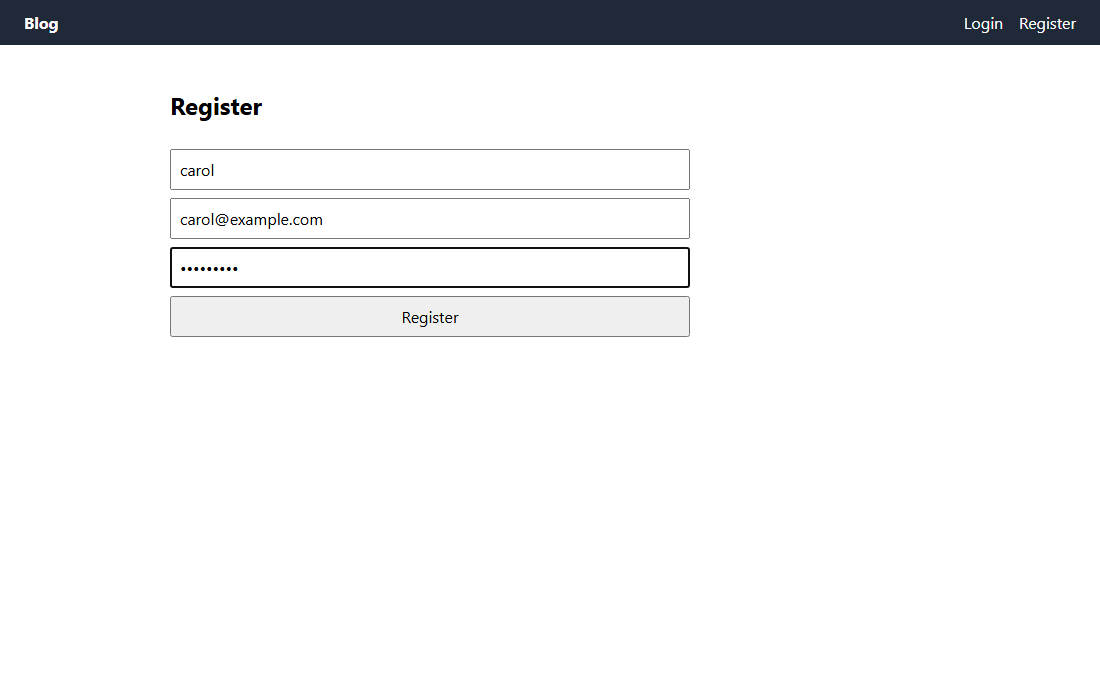
\includegraphics[width=0.85\textwidth]{figures/app-register.png}
\caption{Registration form}
\end{figure}

\begin{figure}[H]
\centering
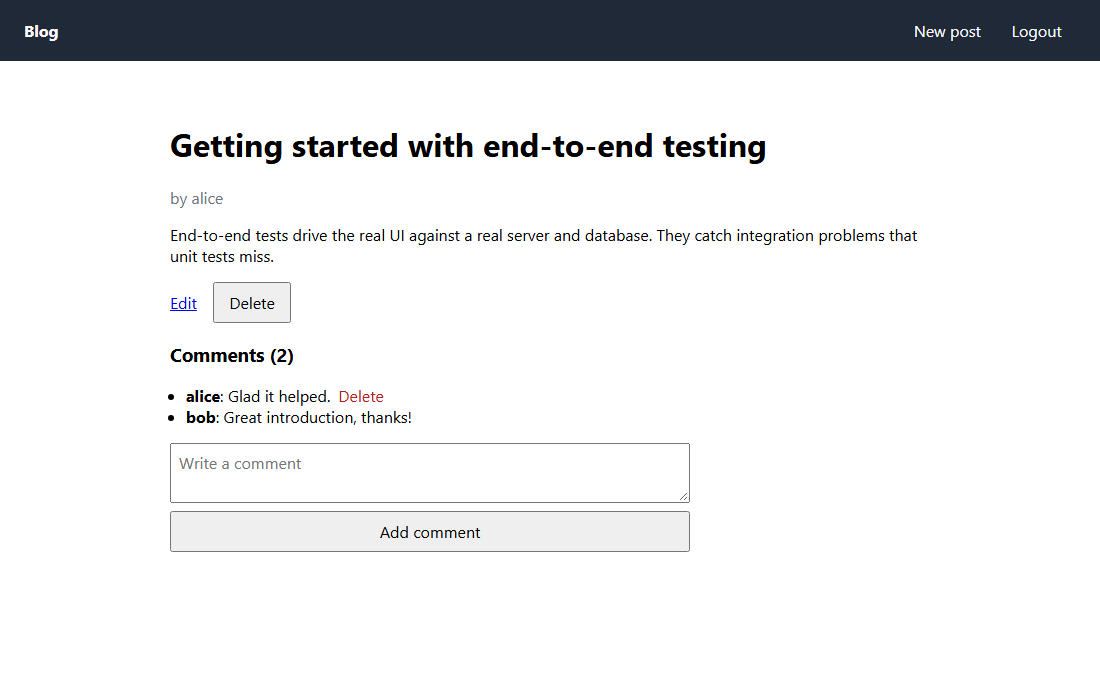
\includegraphics[width=0.85\textwidth]{figures/app-post-author.png}
\caption{A post as seen by its author, with Edit and Delete buttons}
\end{figure}

\begin{figure}[H]
\centering
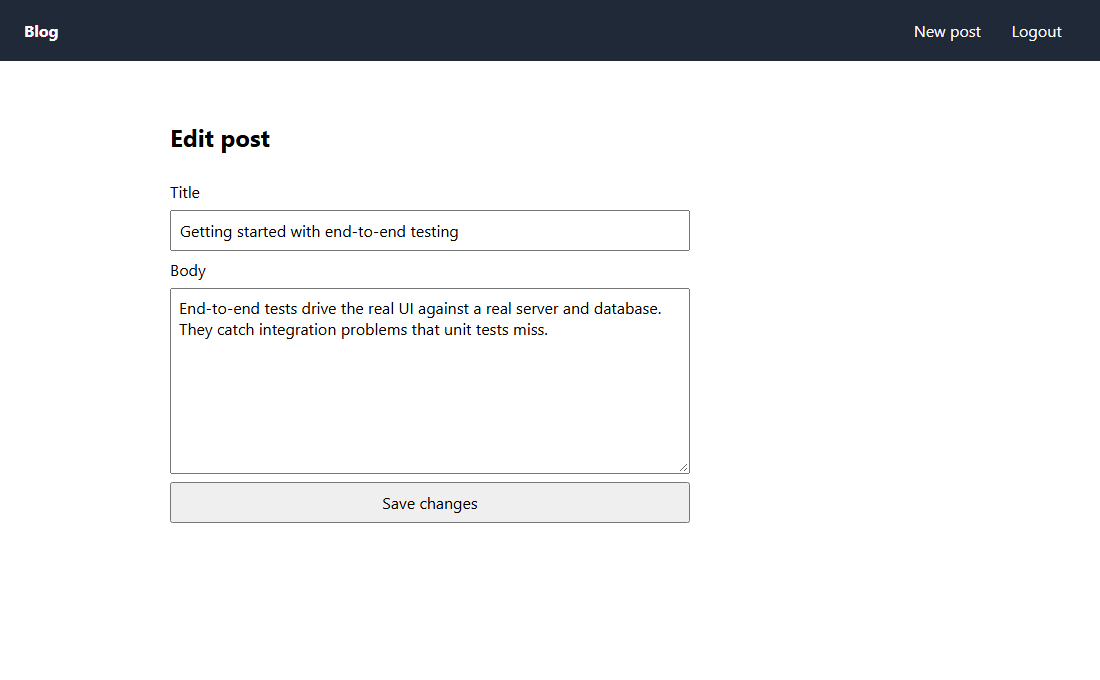
\includegraphics[width=0.85\textwidth]{figures/app-edit-form.png}
\caption{Editing a post}
\end{figure}

\begin{figure}[H]
\centering
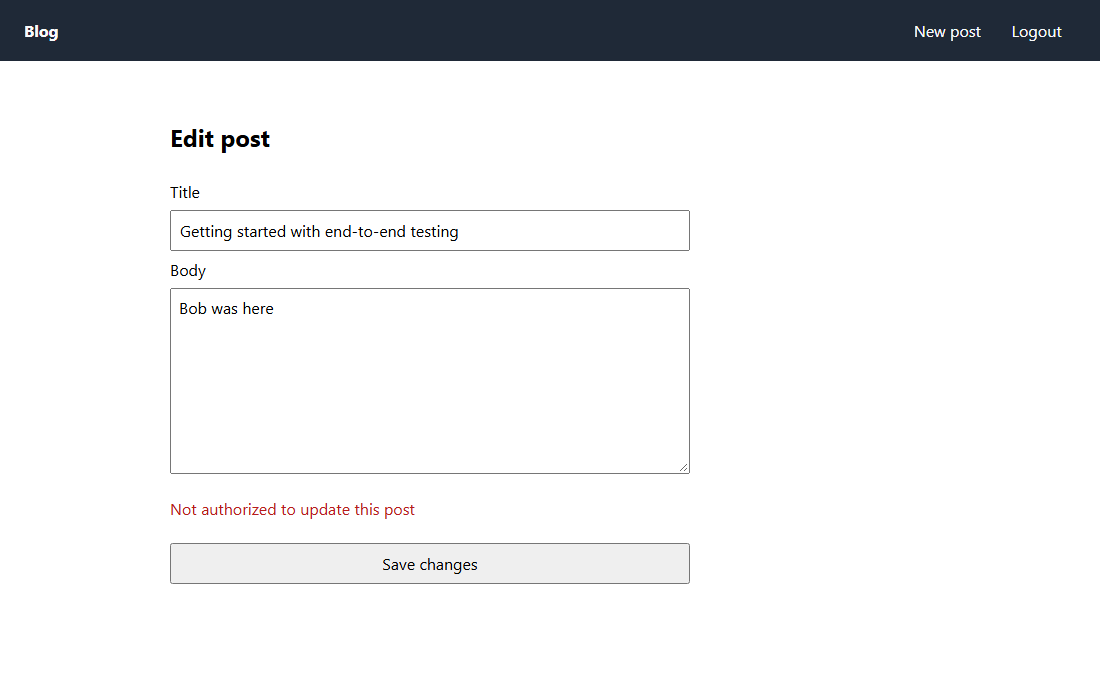
\includegraphics[width=0.85\textwidth]{figures/ses-403-other-user.png}
\caption{TC-SES-06: Bob is logged in and tries to save a change to Alice's post. The server replies with 403.}
\end{figure}

\begin{figure}[H]
\centering
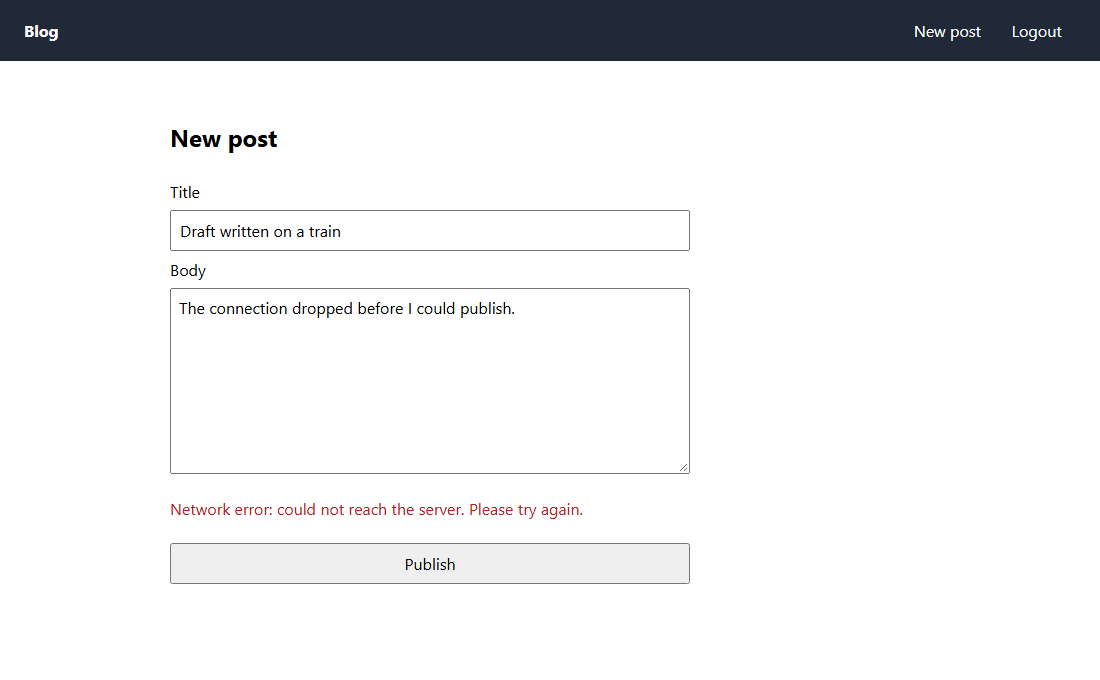
\includegraphics[width=0.85\textwidth]{figures/net-publish-offline.png}
\caption{TC-NET-01: the server cannot be reached, so the user sees an error and the draft is kept}
\end{figure}

\begin{figure}[H]
\centering
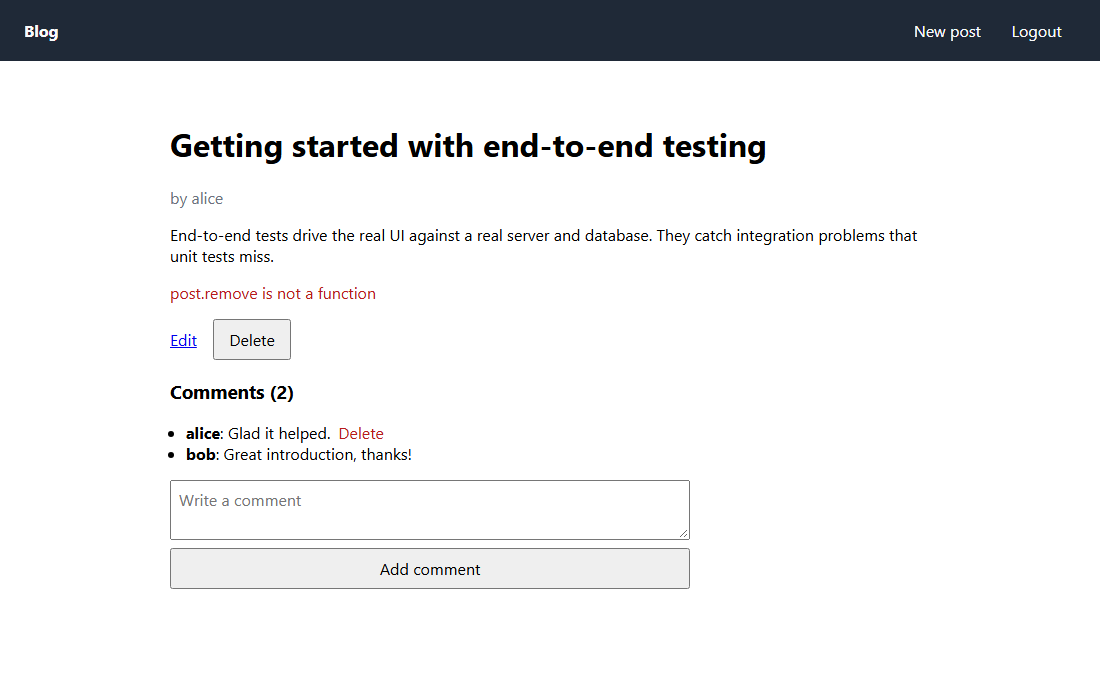
\includegraphics[width=0.85\textwidth]{figures/bug-delete-post.png}
\caption{BUG-01: deleting a post fails with ``post.remove is not a function''}
\label{fig:bugdelete}
\end{figure}

\begin{figure}[H]
\centering
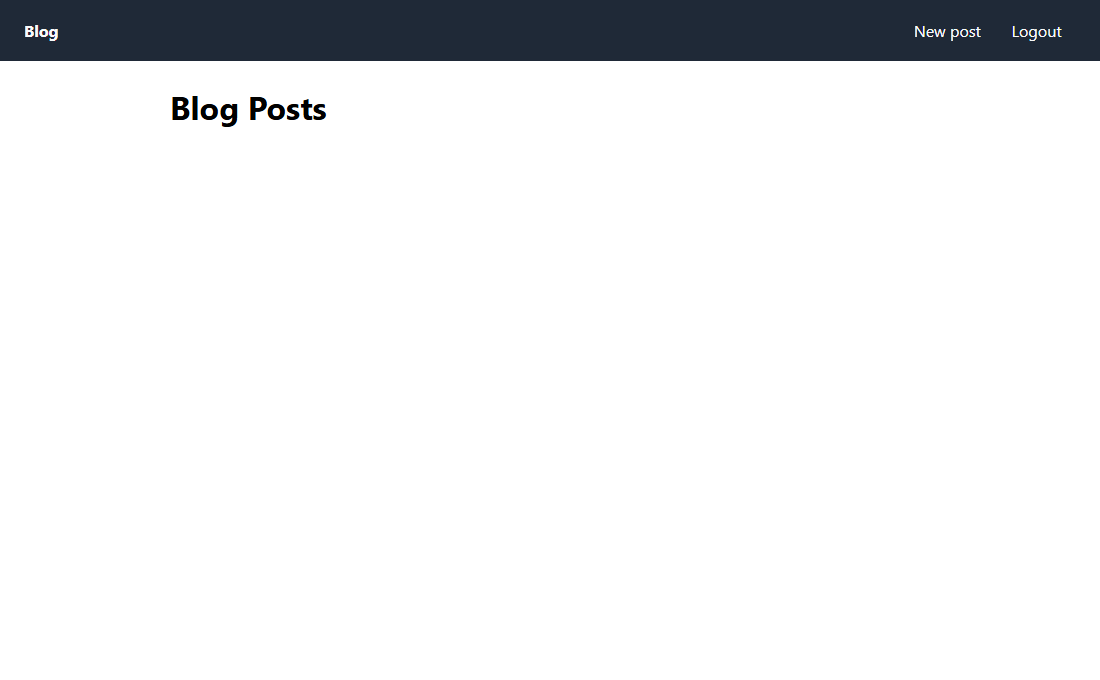
\includegraphics[width=0.85\textwidth]{figures/bug-home-network.png}
\caption{BUG-12: the home page stays empty, with no message, when posts cannot be loaded}
\label{fig:bughome}
\end{figure}

% ================================================================= CHAPTER 9
\chapter{Conclusion}

We tested a MERN blog application from end to end with 48 Playwright test cases
on Chromium, Firefox and WebKit. The tests cover registration and login,
creating and editing posts and comments (with checks in the database), and the
complete flow of publishing, editing and commenting. We used session-data based
testing to write the negative test cases for unauthorized access, and we also
tested network failures and form validation.

Out of 126 test runs, 100 passed (79.4\,\%), and the results were the same on
all three browsers. The main session checks work well. The server rejects
edited, forged, unsigned and expired tokens, and users cannot edit each other's
posts.

The tests also found 12 bugs. Two of them stop users from deleting posts and
comments. Four are security or privacy problems: tokens still work after
logout, error replies show stack traces, anyone can see all users' e-mail
addresses, and a deleted user's token causes a server error. The rest are about
how the server checks input and handles errors. Since our tests check for the
correct behaviour, they can be run again after these bugs are fixed to confirm
the fixes.

\bigskip
\noindent For more details on the project, including the source code,
installation steps and test cases, please refer to the
\href{\repourl}{\fbox{GitHub Repository}}.

% ================================================================= APPENDIX
\appendix
\chapter{Running the Tests}

\begin{lstlisting}[language=bash]
git clone https://github.com/gishee003/Blog-E2E-Testing.git
cd Blog-E2E-Testing

# application
cd app && npm install && cp .env.example .env     # set JWT_SECRET in .env
cd blog-client && npm install && cd ../..

# tests (MongoDB must be running on 127.0.0.1:27017)
cd e2e-tests && npm install
npx playwright install          # downloads Chromium, Firefox and WebKit
npx playwright test             # starts the API and the React build automatically
npx playwright show-report      # opens the HTML report
\end{lstlisting}

\end{document}
